\documentclass[a4paper]{article}

%-----------------------------------------------------
\usepackage[a4paper, total={7in, 9in}]{geometry}
\usepackage{amsmath}
\usepackage{booktabs}
\usepackage{caption}
\usepackage{enumitem}
\usepackage{graphicx}
\usepackage{float}
\usepackage{inconsolata}
\usepackage{listings}
\usepackage{pstricks-add}
\usepackage{siunitx}
\usepackage[most]{tcolorbox}
\usepackage{tikz}
\usepackage{xfrac}
\usepackage{color}
\usepackage{multirow}
\usepackage{rotating}
\usepackage{url}

\usetikzlibrary{arrows}

%-----------------------------------------------------
\graphicspath{{./fig/}}
\setlength{\parindent}{0in}
%-----------------------------------------------------
\begin{document}
\title{ENG405 (Integrated Design Project): Critical Analysis}
\author{Tatyana Maltseva (\textbf{s257346}), Sakon Nadthayai (\textbf{s245002}),\\ and Shane Reynolds (\textbf{s262538})}
\maketitle

\tableofcontents

\newpage

%-----------------------------------------------------
\section{Introduction}

\section{Scope}

%-----------------------------------------------------
\section{Critical Analysis of Hardware}

\subsection{Robot Chassis}
The Pololu Dagu Rover 5 is the robot chassis specified by the client which will make up the final design. The chassis has two principal configurations:
\begin{itemize}
\item \textbf{Four motors, with no tracks:} The four motors drive each of the 4 wheels directly;
\item \textbf{Two motors, with tracked wheels:} The motors drive two wheels directly, and the remaining two wheels are each driven by one of the robot tracks which are attached to the driven wheels
\end{itemize}

A four motor configuration has a manoeuvrability advantage over the two motor configuration. This is especially true when the chassis is fitted with XXXX wheels. The four motor design would also be more powerful. The chassis is fabricated with white plastic and is approximately 245$\si{\milli\meter}$ in length, and 225$\si{\milli\meter}$ in width. The robot clearance is adjustable, meaning that the robot height can be modified according to requirements. Increasing the robot's height allows the robot more capability to navigate unstructured terrain. Figure 1 shows a detailed schematic of the chassis dimensions in the two motor, tracked wheels, configuration. Note that there are holes in the corners of the chassis, which will be used to mount additional hardware for the completed design. Given the limited options for hardware placement, this was not considered a design option, however, consideration was given to using a protective housing for the hardware, or not.  

\begin{figure}[h]
\centering
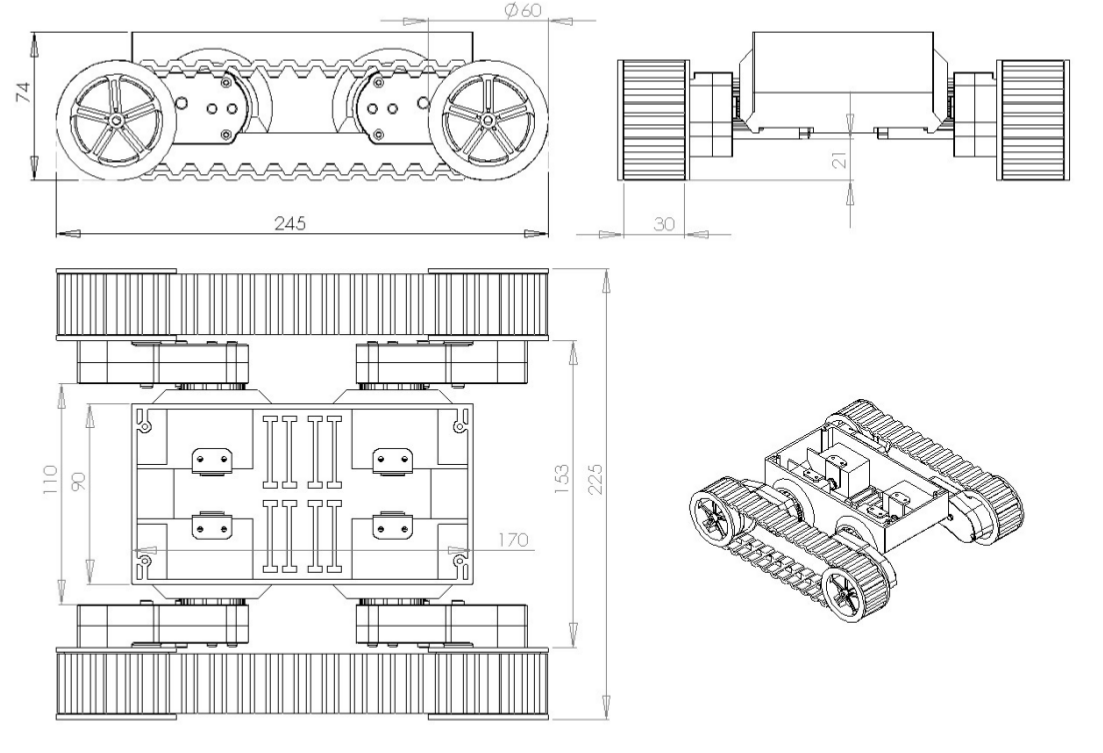
\includegraphics[scale=0.3]{fig1}
\caption{Detailed schematic of the Pololu Dagu Rover 5 chassis, set up with two motors and tracked wheels.}
\end{figure}

%----------------------------------------------------
% Critical Analysis - Do we use the four motor config
% Or do we use the two motor config? Why? Do we adjust
% the height or not? Do we build a housing?
%----------------------------------------------------

There are three main design considerations that need to be analysed in this section:
\begin{enumerate}
\item Should the robot be left in the 2 motor configuration, or changed to the 4 motor configuration? 
\item Should the robot height be adjusted?
\item Should a protective housing for the additional hardware be used?
\end{enumerate}



\subsection{Motors \& Encoders}
Two DC brushed motors are provided with the robot chassis, driving 86.8:1 gearboxes. The full motor specifications can be found in Table 1. Notably, the maximum speed of the motors are 25 $\si{\centi\meter\per\second}$ at 7.2$\si{\volt}$, and both are equipped with 333 CPR encoders.

\begin{table}[h]
\centering
\caption{text}
\footnotesize\begin{tabular}{lp{10cm}}
\toprule
\textbf{Characteristic} & \textbf{Description}\\
\midrule
Voltage & \\
Unloaded Current & \\
Stall Current & \\
Max Speed & \\
\bottomrule
\end{tabular}
\end{table}

Add a description of how the encoders work, and how they could be applied to the task. Then talk about the advantages and disadvantages.

\begin{enumerate}
\item Should the encoders be used or not?
\item What sort of errors will the encoders accumulate if we employ blind odometry?
\item What is the difference between localisation and odemetry in robotics?
\end{enumerate}

\subsection{4 Channel Motor Controller Operation}
\begin{enumerate}
\item What speed should the motors be run at? This means the PWM signal?
\item Should we have variable speed or fixed speed?
\item If we have fixed speed what are the calculations that would determine the inertia of the motor? Does the motor have inertia?
\end{enumerate}
\subsection{Mechanical Push Button Switch}
\subsection{Sensors}
\subsubsection{SHARP GP2Y0A41SK0F IR Sensor}
\subsubsection{Matbotix Ultrasonic Sensor}
\subsubsection{Microsoft 360 Kinect RBGD Camera}

%-----------------------------------------------------
\section{Critical Design Analysis}

\subsection{Design Option 1}
\subsubsection{Hardware \& Operation}
\subsubsection{Software}
\subsubsection{Simulation}

\subsection{Design Option 2}
\subsubsection{Hardware \& Operation}
\subsubsection{Software}
\subsubsection{Simulation}

\subsection{Design Option 3}
\subsubsection{Hardware \& Operation}
\subsubsection{Software}
\subsubsection{Simulation}

%-----------------------------------------------------
\section{Constraints \& Assumptions}

%-----------------------------------------------------
\section{Timeframes}

%-----------------------------------------------------
\section{Budgets}

%-----------------------------------------------------
\section{Recommended Option}


\end{document}